\documentclass{standalone}
\usepackage{tikz}
\usepackage{amsmath}
\usetikzlibrary{patterns,decorations.markings,backgrounds}
\usetikzlibrary{arrows.meta}

\def\a{-20}
\def\d{4}
\def\w{15}
\def\b{55}
\def\scale{0.2}
\def\eps{0.5}
\def\wall{0.5}
\def\h{20}

\def\aa{\a*\scale}
\def\dd{\d*\scale}
\def\ww{\w*\scale}
\def\bb{\b*\scale}
\def\hh{\h*\scale}

\def\textscale{2}

\begin{document}
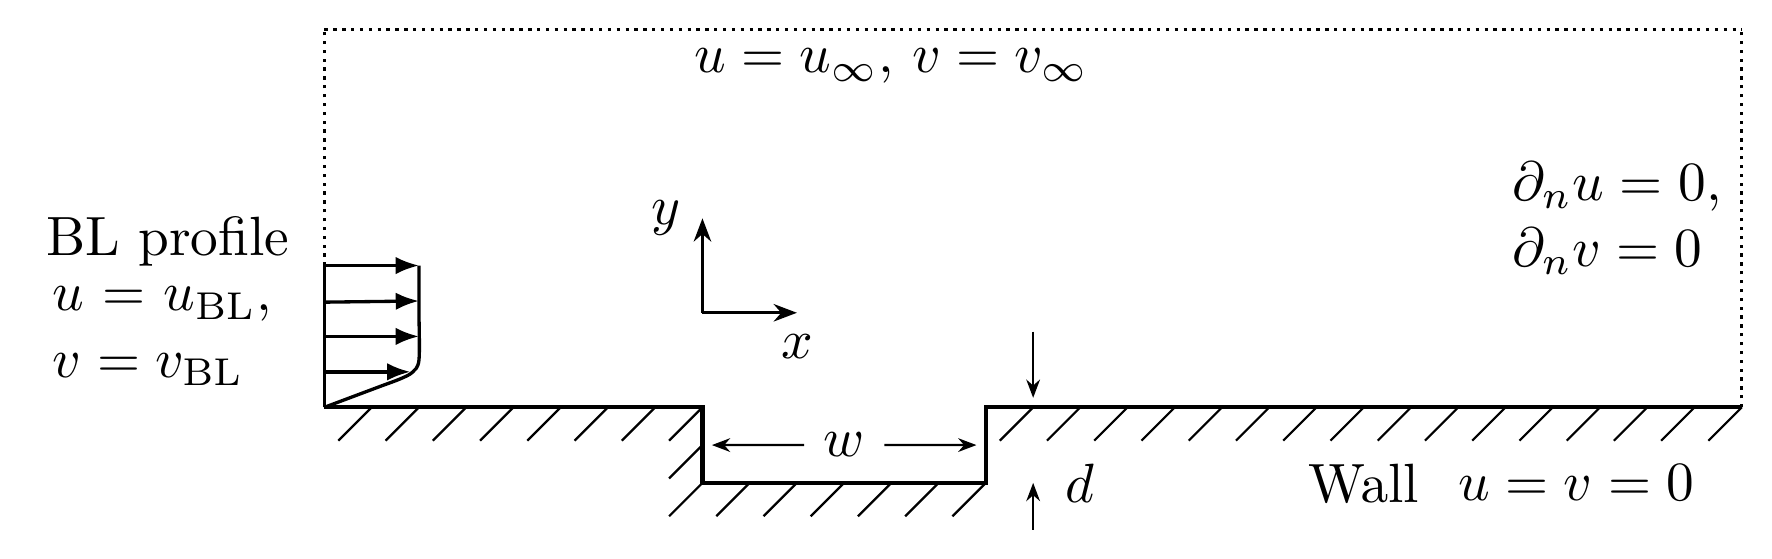
\begin{tikzpicture}[scale=1.2]

% Wall
\draw[ultra thick] (\aa,0) -- (0,0) -- (0,-\dd) -- (\ww,-\dd) -- (\ww,0) -- (\bb,0);

\def\lengthWall{0.5}
\foreach \x in {-3.5,-3,...,0,3.5,4,...,11} {
    \draw[thick] (\x,0) -- ++(225:\lengthWall); % Wall hatching
}
\foreach \x in {0,0.5,...,3} {
    \draw[thick] (\x,-\dd) -- ++(225:\lengthWall); % Wall hatching
}
\draw[thick] (0,-\dd/2) -- ++(225:\lengthWall); % Wall hatching

% BL Profile (velocity profile)
\def\BLxshift{-2cm}
\draw [black, very thick, xshift=\BLxshift] plot [smooth, tension=0.5] coordinates { (-2,0) (-1.8,0.075) (-1.6,0.15) (-1.4, 0.225) (-1.2, 0.3) (-1.07,0.37) (-1,0.5) (-1, 1) (-1,1.25) (-1,1.5)};
\draw [black, very thick, xshift=\BLxshift] (-2,0) -- (-2,1.5); % Left vertical line of BL profile
\draw [-Latex, very thick, xshift=\BLxshift] (-2,1.5) -- (-1,1.5); % Arrow at the top of BL profile
\draw [-Latex, very thick, xshift=\BLxshift] (-2,1.1125) -- (-1,1.125); % Arrow at the middle of BL profile
\draw [-Latex, very thick, xshift=\BLxshift] (-2,0.75) -- (-1,0.75); % Arrow at the bottom of BL profile
\draw [-Latex, very thick, xshift=\BLxshift] (-2,0.375) -- (-1.09,0.375); % Arrow at the bottom of BL profile


% axis orientation
\def\lengthAxis{0.5}
\def\xLocAxis{0}
\def\yLocAxis{0.5}
\draw[-Stealth, very thick,scale=\textscale] (\xLocAxis, \yLocAxis) -- ++(0, \lengthAxis) node[above, anchor=east,scale=\textscale] {$y$}; % y-axis
\draw[-Stealth, very thick,scale=\textscale] (\xLocAxis, \yLocAxis) -- ++(\lengthAxis, 0) node[below, anchor=north,scale=\textscale] {$x$}; % x-axis

% width and depth of the domain
\node[scale=\textscale] (width) at (\ww/2,-\dd/2) {$w$};
% \draw[-Stealth,very thick] (\aa,\hh) -- (\bb,\hh); % Top boundary line
\draw[Stealth-, thick] (0.1,-\dd/2) -- (width.west);
\draw[-Stealth, thick] (width.east) -- (\ww-0.1,-\dd/2); % Width arrow

\node[scale=\textscale] (depth) at (\ww+1, -\dd) {$d$};
\draw[-Stealth,thick] (\ww+0.5,\dd) -- (\ww+0.5,0.1); % Depth arrow
\draw[Stealth-, thick] (\ww+0.5,-\dd) -- (\ww+0.5,-\dd-0.5); % Depth arrow




% Upper region
\draw[dotted,very thick] (\aa,\hh) -- (\bb,\hh); % Top boundary line
\draw[dotted,very thick] (\aa,0) -- (\aa,\hh); % Left boundary line
\draw[dotted,very thick] (\bb,0) -- (\bb,\hh); % Right boundary line

% Labels
\node[scale=\textscale] (W) at (7,-0.8) {Wall};
\node[xshift=\BLxshift,anchor=east,scale=\textscale] at (-2.5,1.75) {BL profile};
\node[xshift=\BLxshift,anchor=east,scale=\textscale,text width=1.5cm] at (-2.5,0.75) {$u=u_\text{BL}$, $v=v_\text{BL}$};
\node[scale=\textscale,anchor=west] at (W.east) {$u=v=0$};
\node[scale=\textscale,anchor=north] at (2,\hh) {$u=u_\infty$, $v=v_\infty$};
\node[scale=\textscale,text width=1.35cm] at (9.7,2) {$\partial_nu=0$, $\partial_nv=0$};

\end{tikzpicture}
\end{document}
